\documentclass[12pt]{article}
\usepackage[a4paper]{geometry}
\usepackage{fullpage}
\usepackage[T1]{fontenc}
\usepackage[utf8]{inputenc}
\usepackage{graphicx}
\usepackage{mathpazo}
\pagenumbering{gobble}
\usepackage{siunitx}
\DeclareSIUnit\voltampere{VA}
\usepackage{amsmath}
\usepackage[spanish]{babel}
\usepackage{steinmetz}

\renewcommand{\thesection}{Problema \arabic{section}}

\begin{document}

\title{}

\date{Marzo 2020}

\section{}

% Una resistencia de \SI{5}{\ohm} y un condensador se unen en serie. La tensión en la resistencia es : $u_R(t) = 25 \cdot \sin(2000t + \pi/6)$. Si la corriente está adelantada \SI{60}{\degree} respecto de la tensión aplicada, ¿cuál es el valor de la capacidad C del condensador?.

% \clearpage

Una resistencia de \SI{5}{\ohm} y un condensador se unen en serie. La tensión en la resistencia es : $u_R(t) = 25 \cdot \sin(2000t + \pi/6)$. Si la corriente está adelantada \SI{60}{\degree} respecto de la tensión aplicada, ¿cuál es el valor de la capacidad C del condensador?.

\begin{equation*}
    \theta = \theta_V - \theta_I \rightarrow \theta = -\pi/3
\end{equation*}

\begin{equation*}
    \overline{Z} = R - j \frac{1}{\omega C R}
  \end{equation*}
  
\begin{equation*}
  \tan \theta = - \frac{1}{\omega C R} \rightarrow \sqrt{3} = \frac{1}{10000 C}
\end{equation*}

\begin{equation*}
  \boxed{C = \SI[parse-numbers = false]{100\sqrt{3}/3}{\micro\farad}}
\end{equation*}

\clearpage


\section{}

% Para determinar las constantes R y L de una bobina, se conecta en serie con una resistencia de \SI{25}{\ohm} y al conjunto se le aplica una fuente de tensión de \SI{120}{\volt} a \SI{60}{\hertz}, se miden las tensiones en bornes de la resistencia y de la bobina, dando los valores $U_R = \SI{70.8}{\volt}$ y $U_B = \SI{86}{\volt}$. ¿ Cuáles son las constantes de la bobina en cuestión?.

% \clearpage

Para determinar las constantes R y L de una bobina, se conecta en serie con una resistencia de \SI{25}{\ohm} y al conjunto se le aplica una fuente de tensión de \SI{120}{\volt} a \SI{60}{\hertz}, se miden las tensiones en bornes de la resistencia y de la bobina, dando los valores $U_R = \SI{70.8}{\volt}$ y $U_B = \SI{86}{\volt}$. ¿ Cuáles son las constantes de la bobina en cuestión?.

\begin{equation*}
  \overline{U} = \overline{U}_B + \overline{U}_R
\end{equation*}



\begin{equation*}
  \overline{U}_R = 25 \overline{I} \rightarrow I = \frac{U_R}{25} = \SI{2.83}{\ampere}
\end{equation*}

\begin{equation*}
  \overline{Z}_B = R_B + j\omega L_B
\end{equation*}

\begin{equation*}
  \overline{U}_B = \overline{I} \cdot \overline{Z}_B \rightarrow 86 = 2.83 Z_B \rightarrow Z_B = \SI{30.37}{\ohm}
\end{equation*}

\begin{equation*}
  \overline{Z} = (25 + R_B) + j\omega L_B
\end{equation*}

\begin{equation*}
  \overline{U} = \overline{I} \cdot \overline{Z} \rightarrow 120 = 2.83 Z \rightarrow Z = \SI{42.37}{\ohm}
\end{equation*}

\begin{align*}
  30.37 &= \sqrt{R^2_B + (\omega L_B)^2}\\
  42.37 &= \sqrt{(25 + R_B)^2 + (\omega L_B)^2}
\end{align*}

\begin{align*}
  R &= \SI{5}{\ohm}\\
  L &= \SI{79.5}{\milli\henry}
\end{align*}

\clearpage


\section{}

% Un circuito serie RLC con $R = \SI{5}{\ohm}$ , $L = \SI{0.02}{\henry}$ y $C=\SI{80}{\micro\farad}$, tiene aplicada una tensión senoidal de frecuencia variable. Determinar los valores de la pulsación $\omega$ para los cuales la corriente:
% \begin{enumerate}
% \item Adelanta \SI{45}{\degree} a la tensión.
% \item Está en fase con ella.
% \item Retrasa \SI{45}{\degree}.
% \end{enumerate}

% \clearpage



Un circuito serie RLC con $R = \SI{5}{\ohm}$ , $L = \SI{0.02}{\henry}$ y $C=\SI{80}{\micro\farad}$, tiene aplicada una tensión senoidal de frecuencia variable. Determinar los valores de la pulsación $\omega$ para los cuales la corriente:
\begin{enumerate}
\item Adelanta \SI{45}{\degree} a la tensión.
\item Está en fase con ella.
\item Retrasa \SI{45}{\degree}.
\end{enumerate}

\begin{equation*}
  \overline{Z} = R + j (\omega L - \frac{1}{\omega C})
\end{equation*}

\begin{equation*}
  \tan \omega = \frac{\omega L - 1/\omega C}{R} = \frac{0.02\omega^2 - 12500}{5\omega}
\end{equation*}

\begin{enumerate}
\item Adelanta \SI{45}{\degree} a la tensión.
  \begin{equation*}
    \theta = -\pi/4 \rightarrow \tan \omega = -1
  \end{equation*}

  \begin{equation*}
    \frac{0.02\omega^2 - 12500}{5\omega} = -1
  \end{equation*}

  \begin{equation*}
    \omega^2 + 250\omega - 625000 = 0 \rightarrow \boxed{\omega = \SI{675}{\radian\per\second}}
  \end{equation*}

  
\item Está en fase con ella.

  \begin{equation*}
    \theta = 0 \rightarrow \tan \omega = 0
  \end{equation*}

  \begin{equation*}
    0.02\omega = \frac{12500}{\omega}
  \end{equation*}

  \begin{equation*}
    \omega = \SI{790.6}{\radian\per\second}
  \end{equation*}
  
\item Retrasa \SI{45}{\degree}.

  \begin{equation*}
    \theta = +\pi/4 \rightarrow \tan \omega = +1
  \end{equation*}

  \begin{equation*}
    \frac{0.02\omega^2 - 12500}{5\omega} = 1
  \end{equation*}

  \begin{equation*}
    \omega^2 - 250\omega - 625000 = 0 \rightarrow \boxed{\omega = \SI{925.4}{\radian\per\second}}
  \end{equation*}

\end{enumerate}

\clearpage

\section{}

% Determinar el triángulo de potencias de un circuito al que se le aplica una tensión $u(t)=340 \cdot \sen(\omega t - 60^\circ)$ V y circula una intensidad de corriente $i(t)= 13.3 \cdot \sen(\omega t-48.7^\circ)$.

% \clearpage

Determinar el triángulo de potencias de un circuito al que se le aplica una tensión $u(t)=340 \cdot \sen(\omega t - 60^\circ)$ V y circula una intensidad de corriente $i(t)= 13.3 \cdot \sen(\omega t-48.7^\circ)$.

\begin{align*}
  \overline{U} &= 170 \sqrt{2}\phase{\ang{-60}}\\
  \overline{I} &= 6.65\sqrt{2}\phase{\ang{-48.7}}
\end{align*}

\begin{equation*}
  \overline{S} = \overline{U}\cdot\overline{I}^* = \SI[parse-numbers=false]{2261\phase{\ang{-11.3}}}{\voltampere}
\end{equation*}


\begin{align*}
  P &= S \cos \theta = \SI{2217.17}{\watt}\\
  Q &= S \sin \theta = \SI{-443.03}{\voltampere_r}
\end{align*}

\clearpage

\section{}


% En el esquema de la figura los elementos tienen los siguientes valores:

% $R_1 = R_2 = R_3 = \SI{10}{\ohm}$

% $X_1 = X_2 = \SI{1}{\ohm}$%

% $R_L = X_L = \SI{1}{\ohm}$

% Sabiendo que $V_{CD} = \SI{200}{\volt}$ se debe calcular:

% \begin{enumerate}
% \item Intensidades de corriente $I$, $I_1$, $I_2$ e $I_3$ \textbf{en forma fasorial}, tomando $V_{CD}$ como referencia de fase.
% \item Lectura de los vatímetros $W_1$ y $W_2$.
% \end{enumerate}

% \begin{center}
%   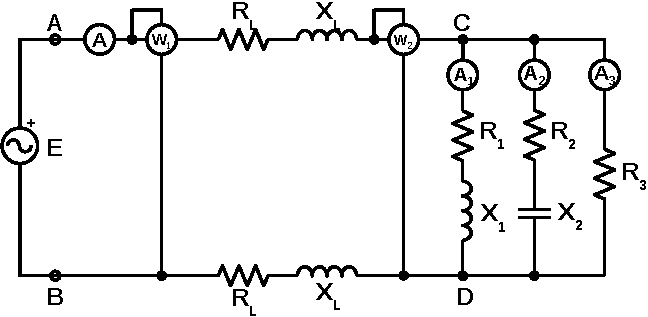
\includegraphics{figs/circuitoA.pdf}
% \end{center}

% \clearpage

En el esquema de la figura los elementos tienen los siguientes valores:

$R_1 = R_2 = R_3 = \SI{10}{\ohm}$

$X_1 = X_2 = \SI{1}{\ohm}$%

$R_L = X_L = \SI{1}{\ohm}$

\begin{center}
  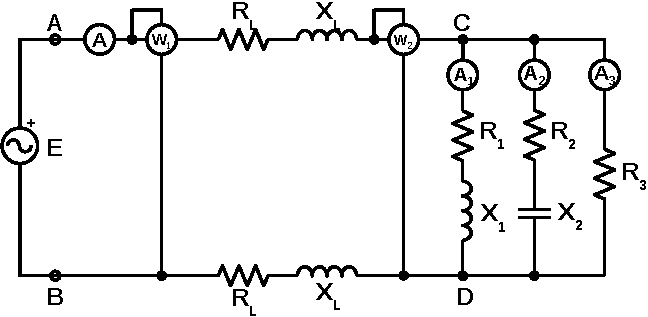
\includegraphics{figs/circuitoA.pdf}
\end{center}

Sabiendo que $V_{CD} = \SI{200}{\volt}$ se debe calcular:

\begin{enumerate}
\item Intensidades de corriente $I$, $I_1$, $I_2$ e $I_3$ \textbf{en forma fasorial}, tomando $V_{CD}$ como referencia de fase.

  \begin{align*}
\overline{V}_{CD} &= \SI[parse-numbers=false]{200\phase{0}}{\volt}\\
%
\overline{Z}_1 &= \SI[parse-numbers=false]{10 + \mathrm{j}}{\ohm}\\
%
\overline{Z}_2 &= \SI[parse-numbers=false]{10 - \mathrm{j}}{\ohm}
\end{align*}

\begin{align*}
\overline{I}_1 &= \frac{\overline{V}_{CD}}{\overline{Z}_1} = \SI[parse-numbers=false]{19.8 - 1.98\mathrm{j}}{\ampere}\\
%
\overline{I}_2 &= \frac{\overline{V}_{CD}}{\overline{Z}_2} = \SI[parse-numbers=false]{19.8 + 1.98\mathrm{j}}{\ampere}\\
%
\overline{I}_3 &= \frac{\overline{V}_{CD}}{R_3} = \SI[parse-numbers=false]{20\phase{\ang{0}}}{\ampere}\\
%
\overline{I} &= \overline{I}_1 + \overline{I}_2 + \overline{I}_3 =  \SI[parse-numbers=false]{59.6\phase{\ang{0}}}{\ampere}\\
\end{align*}

\item Lectura de los vatímetros $W_1$ y $W_2$.

  Calculamos con tensión y corriente:
  \begin{align*}
\overline{S}_2 &= \overline{V}_{CD} \cdot \overline{I}^* = \SI[parse-numbers=false]{11920\phase{\ang{0}}}{VA}\\
%
W_2 &= \mathrm{Re}\{\overline{S}_2\} = \SI{11920}{\watt}
\end{align*}

O mediante teorema de Boucherot:
\begin{align*}
  P_1 = I_1^2 \cdot R_1 &= \SI{3959.6}{\watt}\\
  P_2 = I_2^2 \cdot R_2 &= \SI{3959.6}{\watt}\\
  P_3 = I_3^2 \cdot R_3 &= \SI{4000}{\watt}\\
  W_2 = P = P_1 + P_2 + P_3 &= \SI{11919.2}{\watt}
\end{align*}

Para el vatímetro 1 hay que tener en cuenta la potencia disipada en la línea, y aplicar nuevamente el teorema de Boucherot.
\begin{align*}
P_l &= 2 \cdot I^2 \cdot R_L = \SI{7105.3}{\watt}\\
W_1 &= W_2 + P_l = \SI{19026}{\watt}
\end{align*}

\end{enumerate}

\clearpage

\section{}


% En el circuito los amperímetros $A_1$ y $A_2$ marcan $\SI{4.5}{\ampere}$ y $\SI{6}{\ampere}$, respectivamente; el voltímetro, $\SI{150}{\volt}$ y el
% vatímetro $\SI{900}{\watt}$.

% \begin{center}
%   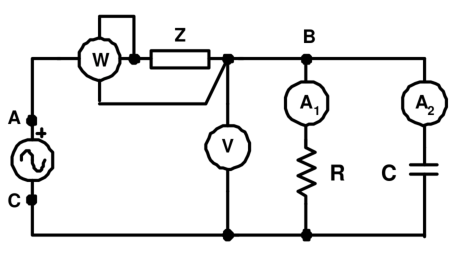
\includegraphics{figs/circuitoZ.pdf}
% \end{center}

% Sabiendo que la frecuencia del generador es de $\SI{250}{\hertz}$ y el f.d.p. de la impedancia $Z$ es de 0.8 en retraso, calcula:
% \begin{enumerate}
% \item Valores de R, C y Z en forma compleja.
% \item Tensión del generador.
% \item Triángulo de potencias totales en forma compleja.
% \end{enumerate}
% \clearpage

En el circuito los amperímetros $A_1$ y $A_2$ marcan $\SI{4.5}{\ampere}$ y $\SI{6}{\ampere}$, respectivamente; el voltímetro, $\SI{150}{\volt}$ y el
vatímetro $\SI{900}{\watt}$.

\begin{center}
  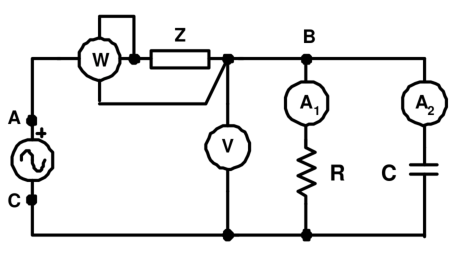
\includegraphics{figs/circuitoZ.pdf}
\end{center}

Sabiendo que la frecuencia del generador es de $\SI{250}{\hertz}$ y el f.d.p. de la impedancia $Z$ es de 0.8 en retraso, calcula:
\begin{enumerate}
\item Valores de R, C y Z en forma compleja.

  \begin{equation*}
    R = \frac{U_{BC}}{A_1} = \frac{150}{4.5} = \SI{33.3}{\ohm}
  \end{equation*}

  \begin{equation*}
    X_c = \frac{U_{BC}}{A_2} = \frac{150}{6} = \SI{25}{\ohm}
  \end{equation*}

  \begin{equation*}
    C = \frac{1}{X_c\omega} = \frac{1}{25 \cdot 2 \pi \cdot 250} = \SI{25.46}{\micro\farad}
  \end{equation*}

  Tomando $\overline{U}_{BC}$ como origen de fases, $\overline{U}_{BC} = \SI[parse-numbers=false]{150\phase{0}}{\volt}$, obtenemos:

  \begin{align*}
    \overline{I}_1 &= \SI[parse-numbers=false]{4.5\phase{0}}{\ampere}\\
    \overline{I}_2 &= \SI[parse-numbers=false]{6\phase{\pi/2}}{\ampere}
  \end{align*}

  Por tanto,
  \[
    \overline{I} = \overline{I}_1 + \overline{I}_2 = \SI[parse-numbers=false]{4.5+6j}{\ampere} = \SI[parse-numbers=false]{7.5\phase{\ang{53.13}}}{\ampere}
  \]
  El vatímetro está midiendo $P_Z = U_Z \cdot I \cos \theta_Z$, y por tanto:

  \[
    U_Z = \frac{900}{7.5 \cdot 0.8} = \SI{150}{\volt}
  \]

  \[
    Z = \frac{U_Z}{I} = \SI{20}{\ohm}
  \]

    También puede obtenerse este resultado calculando primero la parte resistiva de la impedancia:

  \[
    R_Z = \frac{P_Z}{I^2} = \SI{16}{\ohm}
  \]
  y a continuación el módulo teniendo en cuenta que $R = Z \cdot \cos \theta$:

  \[
    Z = \frac{R}{\cos \theta} = \frac{16}{0.8} = \SI{20}{\ohm}
  \]

  Con su factor de potencia obtenemos el ángulo (teniendo en cuenta que es inductiva al ser en retraso), $\theta_Z = \arccos(0.8) = \ang{36.87}$:

  \[
    \overline{Z} = 16 + 12j  = \SI[parse-numbers=false]{20\phase{\ang{36.87}}}{\ohm}
  \]

  
\item Tensión del generador.

  \[
    \overline{U}_{AC} = \overline{U}_{AB} + \overline{U}_{BC}
  \]

  \[
    \overline{U}_{AB} = \overline{Z} \cdot \overline{I} = \SI[parse-numbers=false]{150\phase{\ang{90}}}{\volt}
  \]

  \[
    \overline{U}_{AC} = 150 + 150j = \SI[parse-numbers=false]{150\sqrt{2}\phase{\ang{45}}}{\volt}
  \]

\item Triángulo de potencias totales en forma compleja.

  Podemos calcular a partir de la tensión y la corriente:


  \begin{align*}
    \overline{S}_T &= \overline{U}_{AC} \overline{I}^* =\\
                   &= 150\sqrt{2}\phase{\ang{45}} \cdot 7.5\phase{\ang{-53.13}} =\\
                   &= \SI[parse-numbers=false]{1591\phase{\ang{-8.13}}}{\voltampere}=\\
                   &= \SI[parse-numbers=false]{1575 - j225}{\voltampere}
  \end{align*}
  
  o mediante el teorema de Boucherot:
  \begin{align*}
    P_Z &= \SI{900}{\watt}\\
    P_R = 4.5^2 \cdot 33.3 &= \SI{675}{\watt}\\
    P = P_Z + P_R &= \SI{1575}{\watt}
  \end{align*}

  \begin{align*}
    Q_Z = 7.5^2 \cdot 12 &= \SI{675}{\voltampere_r}\\
    Q_c = - 6^2 \cdot 25 &= \SI{-900}{\voltampere_r}\\
    Q = Q_Z + Q_c &= \SI{-225}{\voltampere_r}
  \end{align*}
  Por tanto:

  \[
    \overline{S} = P + jQ = \SI[parse-numbers=false]{1575 - j225}{\voltampere}
  \]
  
\end{enumerate}


\clearpage

\section{}


% Un motor monofásico de $S = \SI{10}{\kilo\voltampere}$ y $fdp = 0.8$ está alimentado por una fuente de $\SI{230}{\volt}$ a $f = \SI{50}{\hertz}$. 
% Calcula:
% \begin{enumerate}
% \item El valor eficaz de la corriente absorbida por el motor.
% \item La potencia aparente del generador.
% \item La capacidad del condensador necesario para compensar el factor de potencia a la unidad.
% \item El valor eficaz de la corriente absorbida por el conjunto condensador-motor. 
% \item La potencia aparente del generador necesario una vez conectado el condensador del tercer apartado.
% \item Compara de forma razonada los resultados de los apartados 4 y 5 con los valores calculados en los apartados 1 y 2.
% \end{enumerate}

% \clearpage

Un motor monofásico de $S = \SI{10}{\kilo\voltampere}$ y $fdp = 0.8$ está alimentado por una fuente de $\SI{230}{\volt}$ a $f = \SI{50}{\hertz}$. 
Calcula:
\begin{enumerate}
\item El valor eficaz de la corriente absorbida por el motor.
\begin{align*}
  \overline{S}_m &= \overline{V} \cdot \overline{I}^*\\
%
  I &= \frac{\num{10000}}{230} = \SI{43.5}{\ampere}
\end{align*}

\item La potencia aparente del generador.
Suponemos línea ideal (sin perdidas):
\[
  S_g = S_m = \SI{10}{\kilo\voltampere} 
\]

\item La capacidad del condensador necesario para compensar el factor de potencia a la unidad.
\begin{align*}
Q_m &= S \cdot \sin(\theta_m) = \SI{6}{\kilo\voltampere_r}\\
Q_c &= Q_m\\
C &= \frac{Q_m}{\omega \cdot V^2} = \SI{361}{\micro\farad}
\end{align*}

\item El valor eficaz de la corriente absorbida por el conjunto condensador-motor. 
\begin{align*}
Q' &= \SI{0}{\voltampere_r}\\
S' &= P_m = \SI{8}{\kilo\voltampere}\\
I' &= \frac{S'}{V} = \SI{34.8}{\ampere}
\end{align*}

\item La potencia aparente del generador necesario una vez conectado el condensador del tercer apartado.
\begin{align*}
S'_g &= S' = \SI{8}{\kilo\voltampere}\\
\end{align*}

\item Compara de forma razonada los resultados de los apartados 4 y 5 con los valores calculados en los apartados 1 y 2.

  La compensación de reactiva mediante la inserción del condensador ha reducido la corriente que circula por la línea y la potencia del generador en un 20\%.

\end{enumerate}

\clearpage

\section{}


% Un generador de corriente alterna monofásica ($f = \SI{50}{Hz}$) alimenta a dos cargas a través de una línea de cobre. Esta línea, de resistividad $\rho = \SI{0.017}{\ohm\milli\meter\squared\per\meter}$, tiene una longitud de \SI{40}{m} y una sección de \SI{6}{\milli\meter\squared}. Las dos cargas, cuya tensión de alimentación es de \SI{200}{\volt}, son:
% \begin{enumerate}
% \item Un motor de \SI{7}{\kilo\watt} con f.d.p. \si{0,7}.
% \item Un grupo de lámparas fluorescentes con potencia total \SI{200}{\watt} y f.d.p. \si{0,5}.
% \end{enumerate}


% La resolución de este problema incluye: 
% \begin{enumerate}
% \item Esquema del circuito señalando adecuadamente los elementos, corrientes y tensiones.
% \item Potencias activa, reactiva y aparente de cada carga.
% \item Valor eficaz de las corrientes en cada carga, y de la corriente total.
% \item Potencia activa y reactiva entregada por el generador.
% \item Valor eficaz de la tensión en bornes del generador.
% \item Capacidad necesaria a instalar en bornes de las cargas para mejorar el factor de potencia de las mismas a la unidad.
% \item Valor eficaz de la tensión en bornes del generador, y potencia aparente entregada por el mismo una vez instalada la capacidad determinada en el apartado anterior.
% \end{enumerate}

% \clearpage

Un generador de corriente alterna monofásica ($f = \SI{50}{Hz}$) alimenta a dos cargas a través de una línea de cobre. Esta línea, de resistividad $\rho = \SI{0.017}{\ohm\milli\meter\squared\per\meter}$, tiene una longitud de \SI{40}{m} y una sección de \SI{6}{\milli\meter\squared}. Las dos cargas, cuya tensión de alimentación es de \SI{200}{\volt}, son:
\begin{enumerate}
\item Un motor de \SI{7}{\kilo\watt} con f.d.p. \si{0,7}.
\item Un grupo de lámparas fluorescentes con potencia total \SI{200}{\watt} y f.d.p. \si{0,5}.
\end{enumerate}


La resolución de este problema incluye: 
\begin{enumerate}
\item Esquema del circuito señalando adecuadamente los elementos,
  corrientes y tensiones.

    
  \begin{center}
    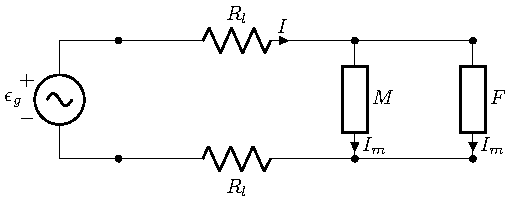
\includegraphics{figs/circuito_cargas.pdf}
  \end{center}
  
\item Potencias activa, reactiva y aparente de cada carga.

\begin{align*}
  P_M &= \SI{7000}{\watt}\\
  Q_M &= \SI{7141.4}{VA}_r\\
  S_M &= \SI{10000}{VA}\\
  P_F &= \SI{200}{\watt}\\
  Q_F &= \SI{346.4}{VA}_r\\
  S_F &= \SI{400}{VA}
\end{align*}

\item Valor eficaz de las corrientes en cada carga, y de la corriente
  total.

  \begin{align*}
    I_M &= S_M / V = \SI{50}{\ampere}\\
    I_F &= S_F / V = \SI{2}{\ampere}
  \end{align*}

  Por teorema de Boucherot la potencia total en cargas es:

\begin{align*}
  P_T &= \SI{7200}{\watt}\\
  Q_T &= \SI{7487.8}{VA}_r\\
  S_T &= \SI{10387.9}{VA}
\end{align*}

Y, por tanto, la corriente total es:
\[
  I = S_T / V = \SI{51.9}{\ampere}
\]

\item Potencia activa y reactiva entregada por el generador.
La resistencia de la línea (una resistencia por cada conductor) es:

\[
R_L = \rho L/S = \SI{0.113}{\ohm}
\]

La potencia activa disipada en la línea es:

\[
P_L = 2 \cdot I^2 R_L = \SI{611.48}{\watt}
\]

Por tanto, la potencia entregada por el generador es:

\begin{align*}
P_g &= P_L + P_T = \SI{7811.5}{\watt}\\
Q_g &= Q_T = \SI{7487.8}{VA}_r\\
S_g &= \SI{10820.7}{VA}
\end{align*}

\item Valor eficaz de la tensión en bornes del generador.
\[
V_g = S_g / I = \SI{208.3}{\volt}
\]

\item Capacidad necesaria a instalar en bornes de las cargas para
  mejorar el factor de potencia de las mismas a la unidad.

  \[
C = \frac{Q_t}{\omega V^2} = \SI{595.9}{\micro\farad}
\]


\item Valor eficaz de la tensión en bornes del generador, y potencia
  aparente entregada por el mismo una vez instalada la capacidad
  determinada en el apartado anterior.

  Una vez instalado este condensador, la corriente total en las cargas es:

\[
I' = P_T / V = \SI{36}{\ampere}
\]

La potencia disipada en la línea es ahora:

\[
P'_L = 2 \cdot I'^2 R_L = \SI{293.8}{\watt} 
\]

Y la potencia entregada por el generador es:
\begin{align*}
P'_g &= \SI{7493.8}{\watt}\\
Q'_g &= \SI{0}{VA}_r\\
S'_g &= \SI{7493.8}{VA}
\end{align*}

Por tanto, la tensión en bornes del generador es:

\[
V'_g = S'_g / I' = \SI{208.2}{\volt}
\]

\end{enumerate}

\clearpage

\section{}
% Un generador de corriente alterna ($f = \SI{50}{\hertz}$) alimenta una instalación eléctrica a través de una línea de cobre ($\rho = \SI{0.017}{\ohm\milli\meter\squared\per\meter}$) de $\SI{25}{\milli\meter\squared}$ de sección. La instalación eléctrica está compuesta por un motor de $S_m = \SI{10}{\kilo\voltampere}$ y $\mathrm{fdp} = 0.8$, una instalación de alumbrado fluorescente de $P_f = \SI{800}{\watt}$ y $\mathrm{fdp} = 0.9$, y diversas cargas electrónicas con una potencia conjunta $P_e = \SI{540}{\watt}$ y $\mathrm{fdp} = 0.5$ en retraso.

% Suponiendo que las cargas trabajan a su tensión nominal de $\SI{230}{\volt}$ y que están situadas a $\SI{100}{\meter}$ del generador, calcule:

% \begin{enumerate}
% \item Triángulo de potencias total de las cargas ($P_T$, $Q_T$, $S_T$) y factor de potencia.
% \item Valor eficaz de la corriente que circula por la línea.
% \item Potencia disipada en la línea.
% \item Triángulo de potencias del generador ($P_g$, $Q_g$, $S_g$) y factor de potencia.
% \item Valor eficaz de la tensión de salida del generador.
% \item Capacidad del banco de condensadores a instalar en bornes de la carga necesario para reducir la corriente que circula por la línea a un valor de $\SI{45}{\ampere}$.
% \end{enumerate}

% Independientemente del resultado obtenido, suponga que la capacidad instalada es $C = \SI{172}{\micro\farad}$. En estas condiciones, calcule:
% \begin{enumerate}
% \item Potencia aparente de las cargas (incluyendo al banco de condensadores)
% \item Valor eficaz de la corriente que circula por la línea y potencia disipada en la misma.
% \item Triángulo de potencias del generador y factor de potencia.
% \item Tensión de trabajo del generador.
% \end{enumerate}

% \clearpage

Un generador de corriente alterna ($f = \SI{50}{\hertz}$) alimenta una instalación eléctrica a través de una línea de cobre ($\rho = \SI{0.017}{\ohm\milli\meter\squared\per\meter}$) de $\SI{25}{\milli\meter\squared}$ de sección. La instalación eléctrica está compuesta por un motor de $S_m = \SI{10}{\kilo\voltampere}$ y $\mathrm{fdp} = 0.8$, una instalación de alumbrado fluorescente de $P_f = \SI{800}{\watt}$ y $\mathrm{fdp} = 0.9$, y diversas cargas electrónicas con una potencia conjunta $P_e = \SI{540}{\watt}$ y $\mathrm{fdp} = 0.5$ en retraso.

Suponiendo que las cargas trabajan a su tensión nominal de $\SI{230}{\volt}$ y que están situadas a $\SI{100}{\meter}$ del generador, calcule:

\begin{enumerate}
\item Triángulo de potencias total de las cargas ($P_T$, $Q_T$, $S_T$) y factor de potencia.

    Motor:
  \begin{align*}
    P_m &= \SI{8000}{\watt}\\
    Q_m &= \SI{6000}{\voltampere}_r\\
  \end{align*}

  Alumbrado
  \begin{align*}
    P_f &= \SI{800}{\watt}\\
    Q_f &= \SI{387.5}{\voltampere}_r\\
  \end{align*}

  Cargas Electrónicas
  \begin{align*}
    P_e &= \SI{540}{\watt}\\
    Q_e &= \SI{935.3}{\voltampere}_r\\
  \end{align*}

  Total (Teorema de Boucherot)
  \begin{align*}
    P_T &= P_m + P_f + P_e = \SI{9340}{\watt}\\
    Q_T &= Q_m + Q_f + Q_e = \SI{7322.8}{\voltampere}_r\\
  \end{align*}

  Por tanto, $S_T = \SI{11868.4}{\voltampere}$ y
  $\mathrm{fdp}_T = 0.787$.

\item Valor eficaz de la corriente que circula por la línea.
\[
  I = \frac{S_T}{U} = \frac{11868.4}{230} = \SI{51.6}{\ampere}
\]

\item Potencia disipada en la línea.

  \begin{align*}
  R &= \SI{0.068}{\ohm}\\
  P_L &= 2 \cdot I^2 \cdot R = \SI{362.1}{\watt}
  \end{align*}

\item Triángulo de potencias del generador ($P_g$, $Q_g$, $S_g$) y factor de potencia.


  \begin{align*}
    P_g &= P_T + P_L = \SI{9702.1}{\watt}\\
    Q_g &= Q_T = \SI{7322.8}{\voltampere}_r\\
    S_g &= \SI{12155.4}{\voltampere}\\    
    \mathrm{fdp} &= 0.798
  \end{align*}

\item Valor eficaz de la tensión de salida del generador.

  \[
    U_g = \frac{S_g}{I} = \SI{235.6}{\volt}
  \]

\item Capacidad del banco de condensadores a instalar en bornes de la carga necesario para reducir la corriente que circula por la línea a un valor de $\SI{45}{\ampere}$.

  Si la corriente en línea se reduce a $\SI{45}{\ampere}$ la potencia aparente resultante en cargas (incluyendo al condensador) es $S'_T = 230 \cdot 45 = \SI{10350}{\voltampere}$. Por tanto, $Q'_T = \SI{4459.5}{\voltampere}_r$. Así, es necesario instalar un banco de condensadores que aporte $Q_c = Q_T - Q'_T = \SI{2863.3}{\voltampere}_r$.

\[
C = \frac{Q_c}{\omega U^2} = \SI{172.3}{\micro\farad}
\]

  
\end{enumerate}

Independientemente del resultado obtenido, suponga que la capacidad instalada es $C = \SI{172}{\micro\farad}$. En estas condiciones, calcule:
\begin{enumerate}
\item Potencia aparente de las cargas (incluyendo al banco de condensadores)
\[
S'_T = \sqrt(P^2_T + Q'^2_T) = \SI{10350.1}{\voltampere}
\]

\item Valor eficaz de la corriente que circula por la línea y potencia disipada en la misma.
\[
I' = \frac{S'_T}{U} = \SI{45}{\ampere}
\]

\[
  P'_L = 2 \cdot I'^2 \cdot R = \SI{275.4}{\watt}
\]

\item Triángulo de potencias del generador y factor de potencia.
  \begin{align*}
    P'_g &= P_T + P'_L = \SI{9615.4}{\watt}\\
    Q'_g &= Q'_T = \SI{4459.5}{\voltampere}_r\\
    S'_g &= \SI{10599.2}{\voltampere}\\    
  \end{align*}

\item Tensión de trabajo del generador.
\[
U'_g = \frac{S'_g}{I'} = \SI{235.5}{\volt}
\]

\clearpage

\section{}

% El circuito de la figura tiene carácter inductivo.  La impedancia de
% linea es $Z=\SI[parse-numbers=false]{10\sqrt{2}}{\ohm}$ con
% f.d.p. $\sqrt{2}/2$ en retraso. 

% Se debe calcular:

% \begin{enumerate}

% \item \textbf{(1p.)} Potencia activa y reactiva consumida por $Z$.

% \item  \textbf{(3p.)} Expresiones complejas de las intensidades medidas por los
%   amperímetros, $I$, $I_1$, $I_2$ e $I_3$. 

% \item  \textbf{(3p.)} Expresiones complejas de las tensiones $U_{AB}$, $U_{AC}$ y
%   $U_{CB}$.

% \item  \textbf{(3p.)} Valores de $R_1$, $X_1$, $R_2$, $R_3$ y $X_3$.

% \end{enumerate}

% Datos:
% \begin{itemize}

% \item Tómese como referencia de fases la intensidad total, $I$.
% \item $A = \SI[parse-numbers = false]{5\sqrt{5}}{\ampere}$.
% \item $A_1 = \SI[parse-numbers = false]{5\sqrt{2}}{\ampere}$.
% \item $A_2 = \SI{5}{\ampere}$.
% \item $A_3 = \SI[parse-numbers = false]{\sqrt{10}}{\ampere}$.
% \item $U_{AB} = \SI{247}{\volt}$
% \item $W_1 = \SI{2350}{\watt}$
% \item $R_1 = R_3$

% \end{itemize}

% \begin{center}
%   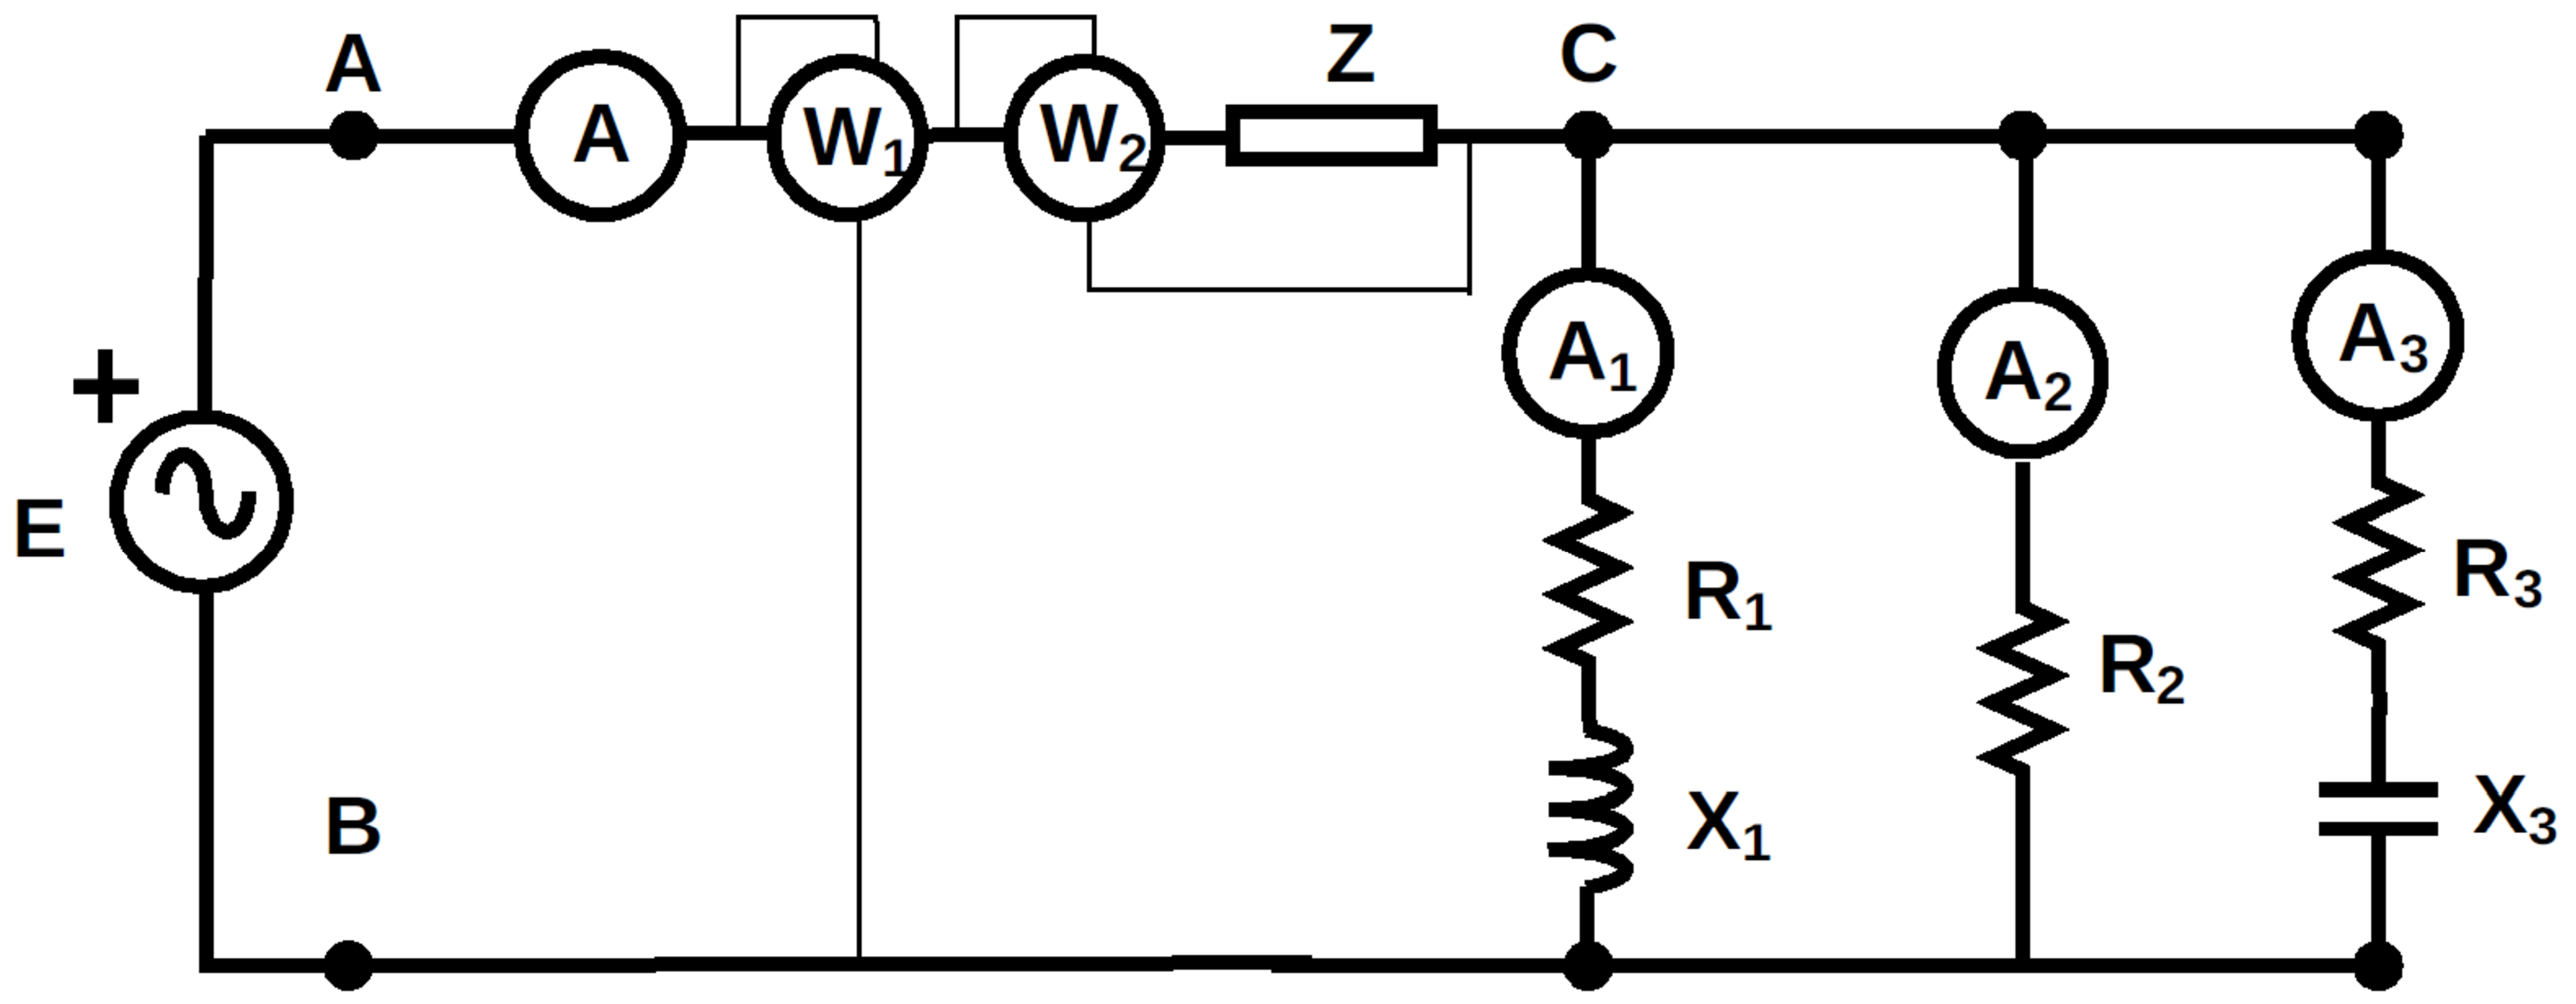
\includegraphics[height=0.2\textheight]{figs/problema10}
% \end{center}

% \clearpage

El circuito de la figura tiene carácter inductivo.  La impedancia de
linea es $Z=\SI[parse-numbers=false]{10\sqrt{2}}{\ohm}$ con
f.d.p. $\sqrt{2}/2$ en retraso. 

Se debe calcular:

\begin{enumerate}

\item \textbf{(1p.)} Potencia activa y reactiva consumida por $Z$.

\item  \textbf{(3p.)} Expresiones complejas de las intensidades medidas por los
  amperímetros, $I$, $I_1$, $I_2$ e $I_3$. 

\item  \textbf{(3p.)} Expresiones complejas de las tensiones $U_{AB}$, $U_{AC}$ y
  $U_{CB}$.

\item  \textbf{(3p.)} Valores de $R_1$, $X_1$, $R_2$, $R_3$ y $X_3$.

\end{enumerate}

Datos:
\begin{itemize}

\item Tómese como referencia de fases la intensidad total, $I$.
\item $A = \SI[parse-numbers = false]{5\sqrt{5}}{\ampere}$.
\item $A_1 = \SI[parse-numbers = false]{5\sqrt{2}}{\ampere}$.
\item $A_2 = \SI{5}{\ampere}$.
\item $A_3 = \SI[parse-numbers = false]{\sqrt{10}}{\ampere}$.
\item $U_{AB} = \SI{247}{\volt}$
\item $W_1 = \SI{2350}{\watt}$
\item $R_1 = R_3$

\end{itemize}

\begin{center}
  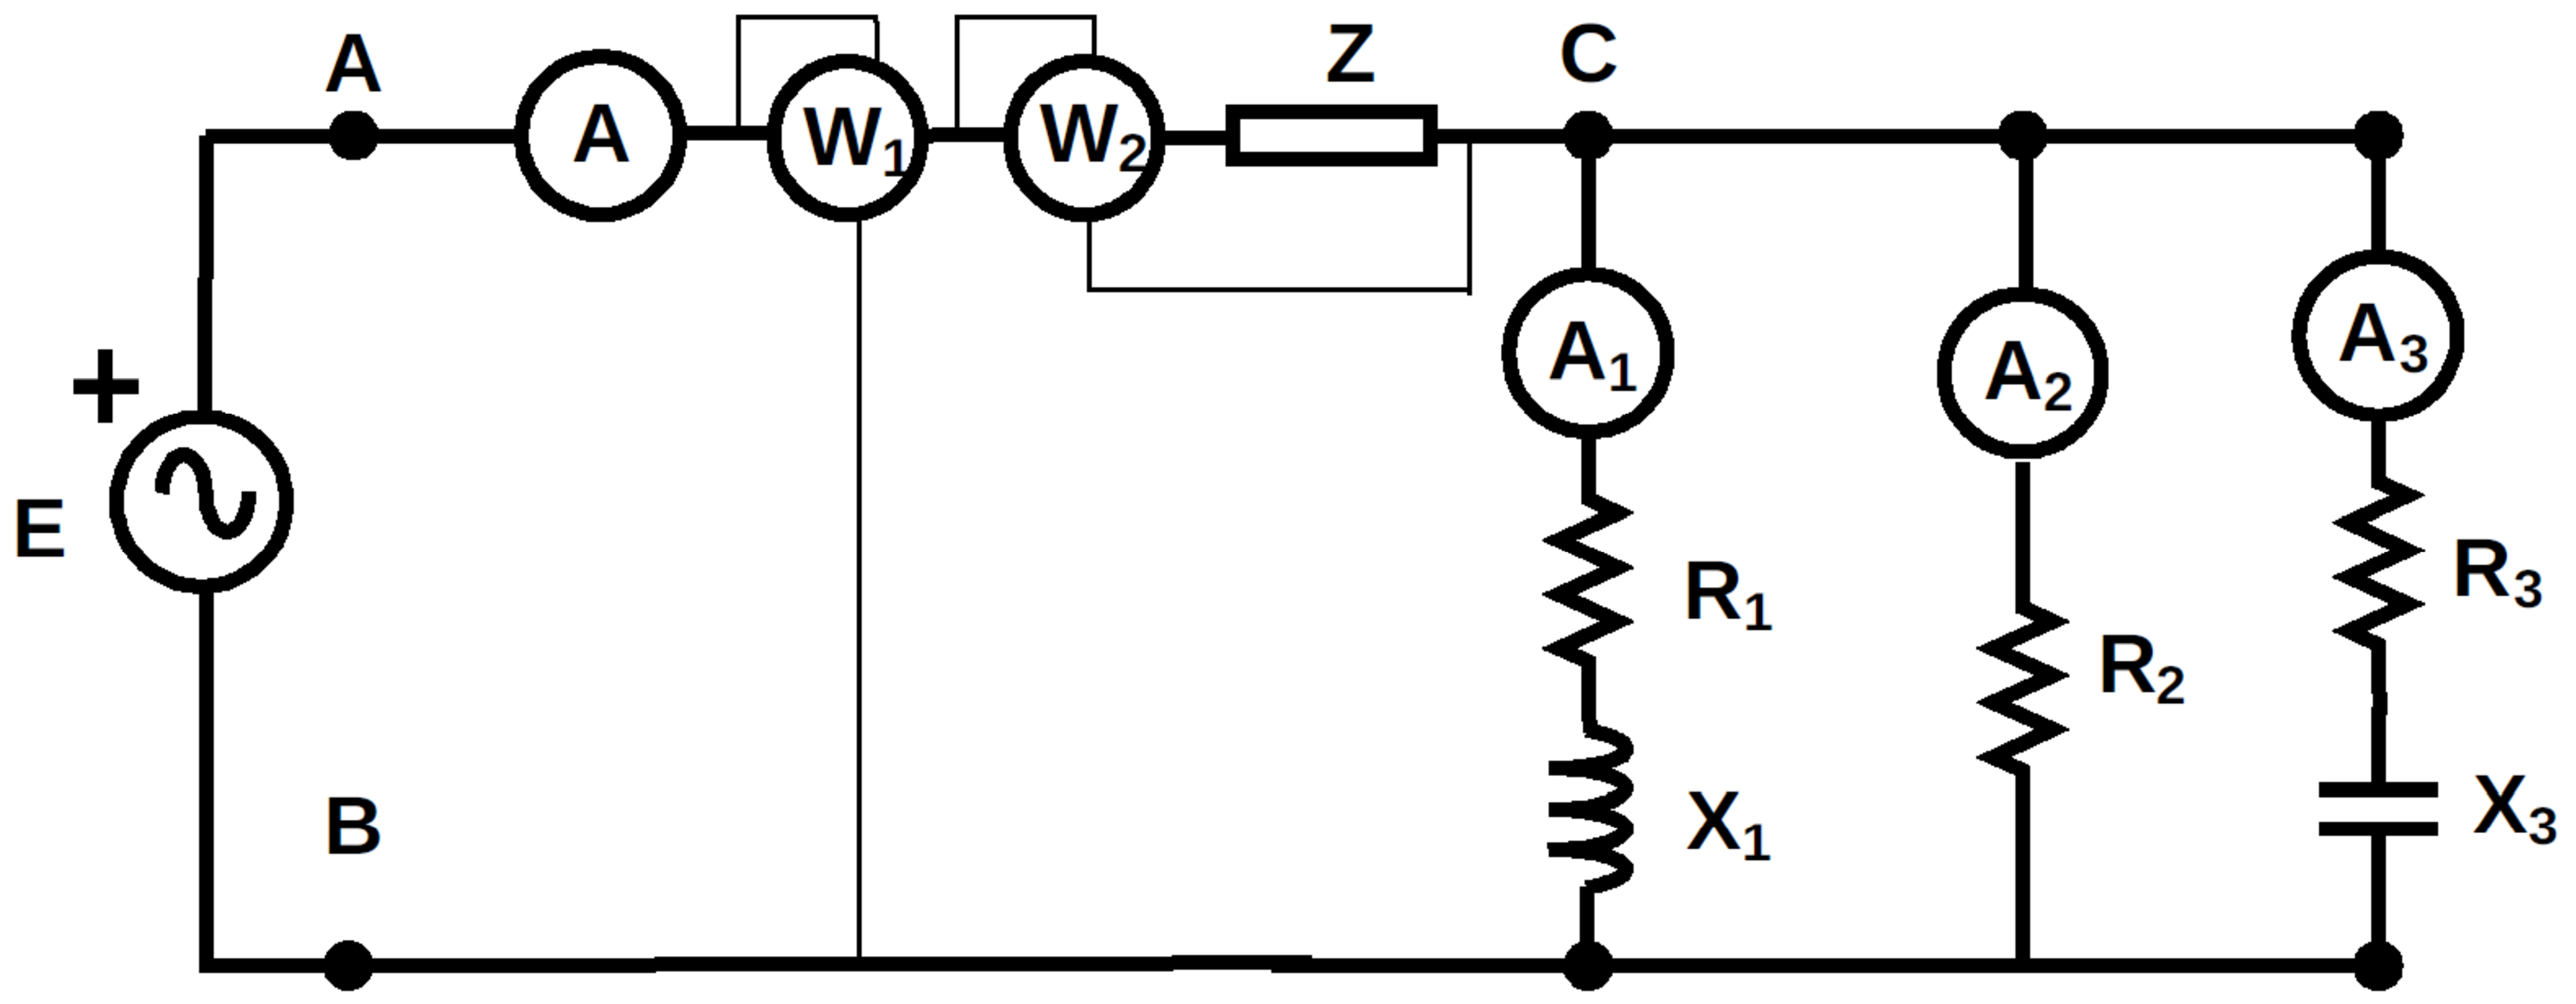
\includegraphics[height=0.2\textheight]{figs/problema10}
\end{center}
Dado que disponemos de la potencia y corriente total y la tensión a
la entrada, podemos calcular el factor de potencia del circuito:

\[
\cos \phi = \frac{P_1}{U_{AB} I} = 0,851
\]

Teniendo en cuenta que la corriente total es la referencia de fases, 

\[
\overline{U}_{AB} = \SI[parse-numbers=false]{247 \phase{\ang{31.68}}}{\V}
\]

También podemos calcular la potencia reactiva del circuito
(positiva dado que el circuito es inductivo):
\[
Q = P \tan \phi = \SI{1450.4}{VA}r
\]


En cuanto a la impedancia $Z$, sabemos que la tensión en sus bornes
es:

\[
\overline{U}_{AC} = \overline{I} \cdot \overline{Z} =
5\sqrt{5}\phase{\ang{0}} \cdot 10\sqrt{2}\phase{\ang{45}} = \SI[parse-numbers=false]{50\sqrt{10}\phase{\ang{45}}}{\V}
\]

Se cumple que $\overline{U}_{AB} = \overline{U}_{AC} +
\overline{U}_{CB}$, y por tanto:

\[
\overline{U}_{CB} = \SI[parse-numbers=false]{100\phase{\ang{10.3}}}{\V}
\]

Por otra parte, podemos descomponer esta impedancia en:
\begin{align*}
  R &= Z \cdot \cos \phi_Z = \SI{10}{\ohm}\\
  X &= Z \cdot \sin \phi_Z = \SI{10}{\ohm}
\end{align*}

y por tanto,

\begin{align*}
P_z &= I^2 \cdot R_z = \SI{1250}{\watt}\\
Q_z &= I^2 \cdot X_z = \SI{1250}{VA}r
\end{align*}

Aplicando el teorema de Boucherot podemos calcular la potencia activa
y la potencia reactiva del circuito paralelo:

\begin{align*}
P_{CB} &= P - P_z = \SI{1100}{\watt}\\
Q_{CB} &= Q - Q_z = \SI{200}{VA}r\\
\overline{S}_{CB} &= P_{CB} + i Q_{CB} = \SI[parse-numbers=false]{1118.03\phase{\ang{10.3}}}{VA}
\end{align*}

Podemos comprobar que estos resultados son coherentes con los
resultados anteriores usando $\overline{S}_{CB} = \overline{U}_{CB}
\cdot \overline{I}^*$.


Ahora podemos obtener $R_2$, $Z_1$ y $Z_3$:

\begin{align*}
  R_2 &= \frac{U_{CB}}{I_2} = \SI{20}{\ohm}\\
  Z_1 &= \frac{U_{CB}}{I_1} = \SI[parse-numbers=false]{10\sqrt{2}}{\ohm}\\
  Z_3 &= \frac{U_{CB}}{I_3} = \SI[parse-numbers=false]{10\sqrt{10}}{\ohm}
\end{align*}

Con los valores de $Z_1$ y $Z_3$ podemos escribir:

\begin{align*}
  Z_1^2 &= R_1^2 + X_1^2 = 200\\
  Z_3^2 &= R_3^2 + X_3^2 = 1000\\
\end{align*}

Por otra parte, la potencia activa del circuito paralelo es:
\begin{align*}
  P_{CB} &= P_1 + P_2 + P_2 =\SI{1100}{\watt}\\
  P_1 &= I_1^2 \cdot R_1 = 50 \cdot R_1\\
  P_2 &= I_2^2 \cdot R_2 = \SI{500}{\watt}\\
  P_3 &= I_3^2 \cdot R_3 = 10 \cdot R_3
\end{align*}

Por tanto, 
\[
   R_1 = R_3 = \SI{10}{\ohm}              
\]

Con este resultado, teniendo en cuenta el módulo de $Z_1$ y $Z_3$,
podemos calcular las reactancias respectivas.

\begin{align*}
  R_1 &= \SI{10}{\ohm}\\
  X_1 &= \SI{10}{\ohm}\\
  \overline{Z}_1 &= 10 + 10i = \SI[parse-numbers=false]{10\sqrt{2}\phase{\ang{45}}}{\ohm}
\end{align*}

\begin{align*}
  R_3 &= \SI{10}{\ohm}\\
  X_3 &= \SI{30}{\ohm}\\
  \overline{Z}_3 &= 10 - 30i = \SI[parse-numbers=false]{10\sqrt{10}\phase{\ang{-71.56}}}{\ohm}
\end{align*}

Podemos comprobar que estas soluciones concuerdan con la potencia
reactiva de cada impedancia y con la total.

\begin{align*}
  Q_1 &= I_1^2 \cdot X_1 = \SI{500}{VA}r\\
  Q_3 &= - I_3^2 \cdot X_3 = \SI{-300}{VA}r\\
  Q_{CB} &= Q_1 + Q_3 =\SI{200}{VA}r
\end{align*}

Con estos resultados, recordando que  $\overline{U}_{CB} =
100\phase{\ang{10.3}}$ podemos calcular las corrientes en forma
compleja:

\begin{align*}
  \overline{I}_1 &=  \SI[parse-numbers=false]{5\sqrt{2}\phase{\ang{-34.7}}}{\ampere}\\
  \overline{I}_2 &=  \SI[parse-numbers=false]{5\phase{\ang{10.3}}}{\ampere}\\
  \overline{I}_3 &=
  \SI[parse-numbers=false]{\sqrt{10}\phase{\ang{81.9}}}{\ampere}
\end{align*}

Para terminar, podemos comprobar que $\overline{I} = \overline{I_1}
+ \overline{I_2} + \overline{I_3}$.
\end{enumerate}

\clearpage{}

\section{}

% En el circuito de la figura, el vatímetro marca $\SI{300}{\watt}$ y el amperímetro $\SI[parse-numbers=false]{\sqrt{2}}{\ampere}$. Se sabe que $X_C = \SI{400}{\ohm}$, y $X_1 = R_1 = 2 \cdot X_2$. La fuente que alimenta el circuito es $e(t) = 200\sqrt{2} \sin(\omega t)$Sabiendo que el factor de potencia del circuito es la unidad, calcula:

% \begin{enumerate}
% \item Valores de $R_1$, $R_2$, $X_1$, $X_2$.
% \item Diagrama fasorial de intensidades.
% \end{enumerate}

% \begin{center}
%   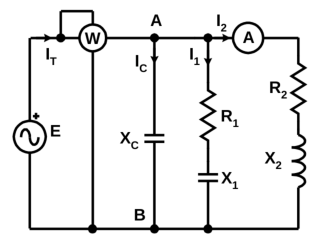
\includegraphics{figs/problema11}
% \end{center}

% \clearpage

En el circuito de la figura, el vatímetro marca $\SI{300}{\watt}$ y el amperímetro $\SI[parse-numbers=false]{\sqrt{2}}{\ampere}$. Se sabe que $X_C = \SI{400}{\ohm}$, y $X_1 = R_1 = 2 \cdot X_2$. La fuente que alimenta el circuito es $e(t) = 200\sqrt{2} \sin(\omega t)$Sabiendo que el factor de potencia del circuito es la unidad, calcula:

\begin{enumerate}
\item Valores de $R_1$, $R_2$, $X_1$, $X_2$.
\item Corrientes $I$, $I_c$, $I_1$, e $I_2$ en forma fasorial. 
\end{enumerate}

\begin{center}
  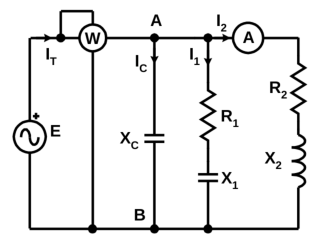
\includegraphics{figs/problema11}
\end{center}


Pasamos a fasores:

\[
  \overline{E} = \SI[parse-numbers=false]{200\phase{0}}{\volt}
\]

Además de la tensión a la entrada, conocemos la lectura del vatímetro, y el factor de potencia del circuito. Podemos, por tanto, calcular la corriente total:

\[
I = \frac{P}{E \cos\theta} = \frac{300}{200} = \SI{1.5}{\ampere}
\]

Dado que $\cos\theta = 1$ y $\theta_V = \ang{0}$, $\overline{I} =  \SI[parse-numbers=false]{1.5\phase{0}}{\ampere}$.

Con la tensión del generador podemos calcular la corriente del condensador:

\[
  I_c = \frac{V_{AB}}{X_c} = \SI{0.5}{\ampere} \rightarrow  \overline{I}_c = \SI[parse-numbers=false]{0.5\phase{\pi/2}}{\ampere}
\]

Para las dos ramas siguientes podemos plantear las siguientes ecuaciones:

\begin{align*}
  \overline{V_{AB}} &= \overline{Z}_1 \cdot \overline{I}_1 = (R_1 - jX_1) \cdot \overline{I}_1\\
  \overline{V_{AB}} &= \overline{Z}_2 \cdot \overline{I}_2 = (R_2 + jX_2) \cdot \overline{I}_2
\end{align*}

Empleando la equivalencia del enunciado, $X_1 = R_1 = 2 \cdot X_2$:

\begin{align*}
   \SI[parse-numbers=false]{200\phase{0}}{\volt} &=  2X_2\cdot (1 - j) \cdot \overline{I}_1\\
   \SI[parse-numbers=false]{200\phase{0}}{\volt} &= (R_2 + jX_2) \cdot \overline{I}_2
\end{align*}

El módulo de la primera ecuación nos proporciona una primera relación útil:

\[
 200 = 2\sqrt{2} X_2 I_1
\]

Por otra parte, mediante el teorema de Boucherot podemos escribir:

\begin{align*}
  P &= I_1^2 R_1 + I_2^2 R_2\\
  Q &= - I_c^2 X_c - I_1^2 X_1+ I_2^2X_2 
\end{align*}

Sustituyendo valores y empleando la relación $X_1 = R_1 = 2X_2$:

\begin{align*}
  300 &= 2I_1^2 X_2 + 2 R_2\\
  0 &= - 1/4 \cdot 400 - 2I_1^2X_2 + 2X_2 
\end{align*}

La última ecuación podemos reescribirla como:

\[
  50 = X_2 \cdot (1- I_1^2)
\]

Teniendo en cuenta la relación entre $X_2$ e $I_1$ que hemos obtenido antes:

\begin{align*}
  50 &= X_2 \cdot (1- I_1^2)\\
  200 &= 2\sqrt{2} X_2 I_1  
\end{align*}
que desemboca en la ecuación:

\[
\sqrt{2} I_1^2 + I_1 - \sqrt{2} = 0 \rightarrow I_1 =  \SI[parse-numbers=false]{\frac{\sqrt{2}}{2}}{\ampere}
\]
y, por tanto:

\begin{align*}
  X_2 &= \SI{100}{\ohm}\\
  X_1 &= \SI{200}{\ohm}\\
  R_1 &= \SI{200}{\ohm}
\end{align*}

Para obtener el valor de $R_2$ recuperamos la ecuación de la potencia activa:

\[
  300 = 2I_1^2 X_2 + 2 R_2 \rightarrow R_2 = \SI{100}{\ohm}
\]

Finalmente, para obtener los fasores de las corrientes $I_1$ e $I_2$ recuperamos las ecuaciones de las dos ramas sustituyendo los valores obtenidos:

\begin{align*}
   \SI[parse-numbers=false]{200\phase{0}}{\volt} &= (200 - j200) \cdot \overline{I}_1\\
   \SI[parse-numbers=false]{200\phase{0}}{\volt} &= (100 + j100) \cdot \overline{I}_2
\end{align*}

\begin{align*}
  \overline{I}_1 &= \SI[parse-numbers=false]{\sqrt{2}/2\phase{\ang{45}}}{\ampere}\\
  \overline{I}_2 &= \SI[parse-numbers=false]{\sqrt{2}\phase{\ang{-45}}}{\ampere}
\end{align*}

\clearpage

\section{}

% La potencia reactiva del circuito de la figura es $\SI{80}{\voltampere_r}$ de tipo capacitivo. La tensión en la impedancia Z está en fase con la intensidad $I_1$ y las lecturas de los aparatos son $A = \SI{4}{\ampere}$, $V = \SI{50}{\volt}$, $W = \SI{200}{\watt}$. Sabiendo que $R_1 = \SI{10}{\ohm}$ y $X_2 = \SI{50}{\ohm}$, calcula:

% \begin{enumerate}
% \item Las corrientes $I_1$, $I_2$, $I_3$ en forma fasorial.
% \item Las reactancias $X_1$, $X_3$, y la impedancia $\overline{Z}$.
% \item La fuerza electromotriz $\overline{E}$.
% \end{enumerate}
% \begin{center}
%   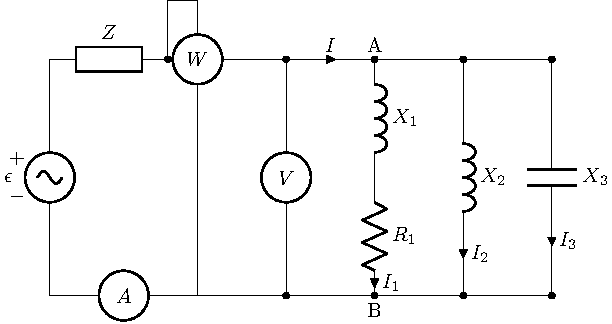
\includegraphics{figs/problema12}
% \end{center}

% \clearpage
La potencia reactiva del circuito de la figura es $\SI{80}{\voltampere_r}$ de tipo capacitivo. La tensión en la impedancia Z está en fase con la intensidad $I_1$ y las lecturas de los aparatos son $A = \SI{4}{\ampere}$, $V = \SI{50}{\volt}$, $W = \SI{200}{\watt}$. Sabiendo que $R_1 = \SI{10}{\ohm}$ y $X_2 = \SI{50}{\ohm}$, calcula:

\begin{enumerate}
\item Las corrientes $I_1$, $I_2$, $I_3$ en forma fasorial.
\item Las reactancias $X_1$, $X_3$, y la impedancia $\overline{Z}$.
\item La fuerza electromotriz $\overline{E}$.
\end{enumerate}
\begin{center}
  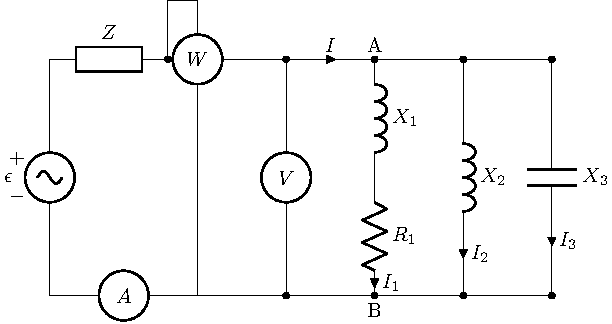
\includegraphics{figs/problema12}
\end{center}

El vatímetro está midiendo la potencia activa del circuito paralelo conectado entre A y B. El único elemento que consume potencia activa en ese circuito es la resistencia $R_1$. Por tanto,

\[
  P_{R1} = 200 = I_1^2 R_1 \rightarrow I_1 = \SI[parse-numbers=false]{2\sqrt{5}}{\ampere}
\]

Dado que conocemos la tensión entre A y B, podemos determinar la impedancia de la rama 1:

\[
  Z_1 = \frac{V_{AB}}{I_1} = \SI[parse-numbers=false]{5\sqrt{5}}{\ohm}
\]
y, por tanto, obtenemos $X_1$:

\[
  Z_1 = \sqrt{R_1^2 + X_1^2} \rightarrow X_1 = \SI{5}{\ohm}
\]

\[
  \overline{Z}_1 = 10 + j5 = \SI[parse-numbers=false]{5\sqrt{5}\phase{\ang{26.56}}}{\ohm} 
\]

Usando la tensión $V_{AB}$ como referencia de fases podemos calcular el ángulo de la corriente $I_1$:

\[
  \overline{I}_1 = \frac{\overline{V}_{AB}}{\overline{Z}_1} = \SI[parse-numbers=false]{2\sqrt{5}\phase{\ang{-26.56}}}{\ampere} 
\]

De la misma forma podemos calcular la corriente $I_2$:
\[
  \overline{I}_2 = \frac{\overline{V}_{AB}}{jX_2} = \SI[parse-numbers=false]{1\phase{\ang{-90}}}{\ampere} 
\]

De la rama 3 no tenemos información directa, luego debemos obtener información del conjunto para aplicarla a esta rama. En particular, del circuito AB conocemos la tensión, la corriente y la potencia, luego podemos obtener su factor de potencia:

\[
  \cos\theta_{AB} = \frac{P_{AB}}{I \cdot V_{AB}} = 1
\]

Por tanto,

\begin{align*}
  Q_{AB} &= 0\\
  \overline{I} &= \SI[parse-numbers=false]{4\phase{\ang{0}}}{\ampere} 
\end{align*}
  
Gracias a este último resultado podemos obtener la corriente en la rama 3:

\[
  \overline{I} = \overline{I}_1 + \overline{I}_2 + \overline{I}_3 \rightarrow \overline{I}_3 = \SI[parse-numbers=false]{3\phase{\pi/2}}{\ampere}
\]

Aplicamos el teorema de Boucherot para obtener reactancia de la rama 3:

\begin{align*}
  Q &= Q_1 + Q_2 + Q_3 = 0\\
  Q_1 &= I_1^2 X_1 = \SI{100}{\voltampere_r}\\
  Q_2 &= I_2^2 X_2 = \SI{50}{\voltampere_r}\\
  Q_3 &= - I_3^2 X_3
\end{align*}

Por tanto,

\[
   Q_3 = -\SI{150}{\voltampere_r} \rightarrow X_3 = \SI[parse-numbers=false]{\frac{50}{3}}{\ohm}
\]

Para determinar $\overline{Z}$ tenemos en cuenta que la potencia reactiva total es $\SI{80}{\voltampere_r}$ de tipo capacitivo y que $Q_{AB} = \SI{0}{\voltampere}_r$:

\[
  Q = Q_Z + Q_{AB} \rightarrow Q_Z = -\SI{80}{\voltampere_r} 
\]

Por tanto:

\[
  X_Z = \frac{|Q_Z|}{I^2} = \SI{5}{\ohm}
\]

Por otra parte, el enunciado indica que la tensión en esta impedancia está en fase con la intensidad $I_1$. Por tanto, $\theta_{VZ} = \ang{-26.56}$, y $\theta_Z = \theta_{VZ} - \theta_{I} = \ang{-25.56}$. Con este ángulo podemos calcular el valor de la resistencia:

\[
  R_Z = \frac{X_Z}{|\tan\theta_Z|} = \SI{10}{\ohm}
\]

\[
  \overline{Z} =  \SI[parse-numbers=false]{10 - j5}{\ohm}
\]

Finalmente, para calcular la fuerza electromotriz podemos hacerlo de dos formas, mediante potencias o mediante tensiones:

Mediante el teorema de Boucherot calculamos la potencia activa:
\[
P = P_Z + P_{AB} = I^2 R_Z + 200 = \SI{360}{\watt}
\]
Y con la potencia reactiva $Q$ obtenemos la potencia aparente:

\[
  \overline{S} = P + jQ = \SI[parse-numbers=false]{360 -j80}{\voltampere}
\]
y la tensión:

\[
  \overline{E} = \frac{\overline{E}}{\overline{I}^*} = 90 - j20 = \SI[parse-numbers=false]{10\sqrt{85}\phase{\ang{-12.53}}}{\volt}
\]

Podemos llegar a este mismo resultado con un balance de tensiones:

\[
  \overline{E} = \overline{V}_Z + \overline{V}_{AB} = \overline{Z} \cdot \overline{I} + \overline{V}_{AB}
\]

\end{document}





